\documentclass[journal]{IEEEtran}
\usepackage{cite}
\usepackage{amsmath,amssymb}
\usepackage{graphicx}
\usepackage{booktabs}
\usepackage{multirow}
\usepackage{url}
\usepackage[hidelinks]{hyperref}
\graphicspath{{figures/}}

\begin{document}

\title{Component Scores Do Not Compose: Clause Detection, Span
Extraction and Category-Level Risk Prioritization on the
Contract Understanding Atticus Dataset}

\author{Jerin Aktar, Afnan Mazumdar, Shoyeb Hasan Sayem and Utsha Kumar Roy}

\markboth{BRAC UNIVERSITY CSE THESIS --- IEEE-FORMAT MANUSCRIPT}%
{BRAC UNIVERSITY CSE THESIS --- IEEE-FORMAT MANUSCRIPT}

\maketitle

\begin{abstract}
Automated contract review is usually evaluated one component at a time. We report a three-stage
pipeline on the Contract Understanding Atticus Dataset (CUAD; 510 contracts, 41 clause categories)
under a contract-level 80/20 split, and three ways component scores misled us. First, a
sliding-window DistilBERT trained under multiple-instance learning lost to a full-document TF--IDF
baseline at clause presence classification (micro-F1 0.692 against 0.775), and the gap survived
controls for training data, random seed, aggregation rule and threshold. Every one of those runs
shared a flaw: a 256-token limit let the model read only 49.3\% of each window. With the whole
window read and both models tuned on the same validation split, the transformer ties the tuned
baseline (0.797 against 0.785) and their ensemble beats it (0.809; lead $+0.024$, 95\% CI
$[+0.011,+0.037]$); a length-only control shows the whole window adds $+0.036$ to the tuned transformer. Second, micro-F1 and the system's purpose diverge: in both setups the configuration ranked
first on micro-F1 misses the most high-risk clauses, while a recall-first configuration chosen on
validation finds 90.3\% of them. Third, stage-wise scores do not compose: only 22.1\% of gold
clauses first survived all stages, against about 77\% predicted. Reading the whole window and
retraining the span model on the chunks it reads at run time raise this to 59.6\%. A 41-template reference set turns plain-language
generation into classification (ROUGE-L 0.775 against the templates, 0.116 against clause-specific
references), and isotonic calibration lowers the presence score's expected calibration error
from 0.206 to 0.016.
\end{abstract}

\begin{IEEEkeywords}
Legal natural language processing, contract analysis, CUAD, multiple-instance learning, model
evaluation, calibration, risk prioritization, held-out evaluation.
\end{IEEEkeywords}

\section{Introduction}
\IEEEPARstart{C}{ommercial} contracts routinely run to tens of thousands of characters, while the
provisions that determine a signer's exposure occupy a few hundred. In CUAD~\cite{cuad} the median
contract is 33,143 characters and the median annotated clause is 196, so the document exceeds a
standard transformer window by roughly $16\times$ while the target sits two orders of magnitude
below it. CUAD frames the resulting task as extraction: given a category, locate the clause. It
stops there, offering no indication of what a located clause means for the party signing it.

This paper reports a system that attempts the further step, and an evaluation of where that system
fails, including one failure in our own first setup. Our contributions are:

\begin{enumerate}
\item A controlled comparison in which a strong lexical baseline looked unbeatable until we found
that the transformer read only half of each window. Once both models read their full input and are
tuned on the same validation split, they tie and their ensemble wins; a length-only control
separates the window effect from the tuning effect (Sections~\ref{sec:controls}
and~\ref{sec:v2}).
\item Evidence that aggregate micro-F1 and user harm can invert the model ranking, measured through
a risk-weighted evaluation, and resolved by fixing a recall-first objective before testing
(Section~\ref{sec:risk}).
\item A demonstration that stage-wise scores do not compose: 22.1\% end-to-end survival against
about 77\% predicted, decomposed into two causes; the full-window presence model and a span model
retrained on the chunks it actually reads raise survival to 59.6\% (Section~\ref{sec:e2e}).
\item A demonstration that a small reference set converts a generation task into classification
without the metric registering the change (Section~\ref{sec:summ}).
\end{enumerate}

\section{Related Work}
CUAD~\cite{cuad} supplies 510 commercial contracts with expert annotations over 41 clause
categories, posed in SQuAD format~\cite{squad}. Domain-adapted encoders~\cite{legalbert} and
benchmark suites~\cite{lexglue} have advanced legal language understanding, but they operationalize
importance as category membership rather than as severity for a particular party. We are not aware
of an established risk-severity model covering CUAD's categories, so the layer added here assigns a
level to each category and makes no claim about the wording of an individual clause.

Long inputs are handled by retrieval, by windowing with aggregation, or by sparse
attention~\cite{longformer}. Windowing aggregated with a maximum is the classical multiple-instance
learning (MIL) rule~\cite{mil}. For generation, T5~\cite{t5} and its instruction-tuned
variant~\cite{flan} express clause simplification naturally; Manor and Li~\cite{manor} assemble
plain-English contract summaries and observe a tendency toward generic output. A substantial
literature establishes that fluent abstractive output is frequently unfaithful~\cite{maynez,factcc}
and that overlap metrics such as ROUGE~\cite{rouge} correlate poorly with faithfulness judgements;
embedding metrics~\cite{bertscore} improve similarity estimation without testing factuality. The
summarization result reported here is an extreme instance of the same phenomenon, and the
calibration analysis follows~\cite{calibration}.

Two properties of CUAD dominate any modelling effort on it. The first is class imbalance:
per-category positive rates span 100\% to 2.5\%. The second is length, which forces every system to
commit to a length strategy before it commits to a model. That choice is usually asserted; here it
is measured, both as a retrieval ceiling obtained before training and as a cost benchmark for
sparse attention on the target hardware.

\section{Proposed Methodology}

\subsection{Pipeline Overview}
The system is a staged pipeline. Contract text is windowed; a presence stage decides which of the
41 categories the contract contains; a span stage extracts the clause text for each detected
category; a risk layer attaches the detected category's level; and a text-generation stage attaches
a plain-English sentence. Each stage is trained independently and, in conventional practice, would
be evaluated independently.

\subsection{Stage 1: Presence Classification}
A TF--IDF representation over the entire document feeds per-category logistic regression, giving a
baseline with no length limit. In parallel, 2,000-character windows at a 1,500-character stride tile
each contract and a DistilBERT~\cite{distilbert} scores (category question, window) pairs; the
document-level score is the maximum over windows, which is the MIL decision rule. The
500-character overlap exceeds the median clause length, so no clause can fall between two windows.
The two models are combined by an AND rule (report a clause only when both fire), an OR rule, the
average of the two scores, or a mixed rule that uses OR for High-risk categories and AND for the
rest.

Before any training we measured the ceiling a retrieval design would impose. The best query
strategy places the gold clause inside its selected windows only 64.0\% of the time, below the
baseline's recall of 0.81, so retrieval was rejected on a measurement rather than an assumption.
The claim is narrow: it bounds \emph{lexical} retrieval only, and a dense retriever may well raise
it.

\subsection{Stage 2: Span Extraction}
\label{sec:stage2}
A DistilBertForQuestionAnswering head predicts start and end token positions. At training time each
example is re-centred so the answer begins approximately 150 characters into a 1,200-character
window, which guarantees the target survives tokenizer truncation. This uses a label to construct a
training example and never to construct an inference input; Section~\ref{sec:e2e} shows it
nevertheless has a cost. A second span model is therefore trained on the inputs it sees at run time:
the presence model's 2,000-character window cut into 1,200-character chunks at offsets 0 and 800.
A chunk that contains the start of a clause is labelled with its true position, wherever it falls;
a chunk that does not is labelled ``no answer'' on [CLS], as in SQuAD~2.0~\cite{squad2}.

\subsection{Risk Prioritization, Plain Language and Calibration}
Each category carries a fixed High/Medium/Low level scored from the weaker party's perspective
(8/22/11) using five criteria: financial exposure, irreversibility, restriction of future freedom,
asymmetry, and survival beyond termination. This is category-level prioritization, not clause-level
assessment: it cannot distinguish a \$10,000 liability cap from a \$10,000,000 one. A FLAN-T5-small
is fine-tuned to map a clause to a plain-English sentence, seeded with 41 author-written category
templates. Finally, an isotonic map fitted on validation contracts converts the max-pooled
presence score into the observed share of contracts that contain the clause; the deployed
application shows this calibrated value instead of the raw score.

\section{Experimental Setup}

\subsection{Dataset and Split}
All experiments use CUAD v1. The split is drawn \textbf{at the contract level}, 80/20, with a fixed
seed: 408 training and 102 test contracts, or 20,910 (contract, category) rows. The same split is
loaded from disk by every model, so ``test'' denotes the same 102 unseen contracts throughout: 4,182
test decisions, 1,348 of them positive. Five categories have at most seven positive test contracts.
For the second setup below, 81 of the 408 training contracts (seed 42) are held out as a validation
split and the models are trained on the remaining 327.

\subsection{Two Setups}
\label{sec:setups}
\emph{First setup.} The presence transformer reads each (question, window) pair up to 256 tokens and
trains on a balanced sample of 24,000 of the 53,662 available training windows. No hyperparameter is
tuned: learning rates, batch sizes and epochs are published defaults, and every decision threshold
is 0.5. This protects the held-out evaluation, but it pits a transformer at an unchosen operating
point against a baseline with almost nothing to tune.

\emph{Re-run.} The input limit is raised to 512 tokens, which covers the question and the whole
window. The transformer trains for three epochs and keeps the epoch with the lowest validation loss.
Both models are then tuned on the 81 validation contracts in the same way: the baseline's
regularization strength $C\in\{0.1,0.3,1,3,10\}$; the transformer's pooling rule (maximum, or mean
of the top 2, 3 or 5 windows); one shared threshold per model, then a per-category threshold for
each category with at least eight validation positives; and the ensemble rule among AND, OR,
average and mixed. Every choice is made twice, once to maximize micro-F1 and once to maximize
micro-F2, which counts a missed clause as worse than a false alarm. The test set is scored once per
finished configuration. A control run repeats the whole protocol with the input left at 256 tokens,
so that input length is the only difference.

\subsection{Evaluation Metrics and Uncertainty}
Presence is scored by micro-F1 (and micro-F2) over the 4,182 test decisions. Because the 41
decisions within a contract are not independent, intervals come from a cluster bootstrap that
resamples \emph{contracts} with replacement (10,000 resamples), not individual cells, and model
comparisons are paired on the same resample. Span extraction is scored by token-level F1 against the
annotated span. Generation is scored by ROUGE-L against two different reference sets, described in
Section~\ref{sec:summ}. Calibration is scored by Expected Calibration Error (ECE) and Brier score.

\subsection{Implementation and Reproducibility}
Training ran on a single Apple M4 laptop with 16\,GB of unified memory using the Metal backend; no
CUDA was used at any point. The split, the validation split, the fitted baselines, all checkpoints,
the chosen thresholds and a standalone evaluation notebook are saved to disk, and a verification
script checks the reported numbers against the stored result files.

\section{Results and Discussion}

\subsection{Presence Classification: First Setup}
Table~\ref{tab:presence} reports micro-F1 over the 4,182 test decisions. The windowed transformer
loses to the lexical baseline by 0.082; the cluster bootstrap places that gap at $[+0.0647,+0.1013]$,
and the baseline wins in every resample. The AND ensemble finishes nominally first at 0.779, with a
margin of $+0.0042$ and an interval of $[-0.0037,+0.0115]$: a tie.

\begin{table}[!t]
\caption{Presence models, first setup, held-out micro-F1}
\label{tab:presence}
\centering
\begin{tabular}{lccc}
\toprule
\textbf{Model} & \textbf{micro-F1} & \textbf{Prec.} & \textbf{Rec.}\\
\midrule
AND ensemble           & \textbf{0.779} & 0.774 & 0.784\\
TF--IDF baseline       & 0.775 & 0.742 & 0.810\\
Ensemble AVG           & 0.718 & --- & ---\\
Transformer (max-pool) & 0.692 & 0.558 & 0.913\\
Ensemble OR            & 0.692 & --- & ---\\
\bottomrule
\end{tabular}
\end{table}

\subsection{Robustness Controls}
\label{sec:controls}
A bootstrap answers whether a gap could be sampling noise; it cannot answer whether the model was
handicapped. Table~\ref{tab:controls} reports the controls we ran on the first setup, and the one
that finally explained the gap.

\begin{table}[!t]
\caption{Explanations for the first-setup transformer's deficit}
\label{tab:controls}
\centering
\small
\setlength{\tabcolsep}{3pt}
\begin{tabular}{lcc}
\toprule
\textbf{Control} & \textbf{Effect on micro-F1} & \textbf{Verdict}\\
\midrule
All 53,662 windows   & $-0.0004$ $[-0.0098,+0.0095]$ & none\\
Random seed, 3 runs  & SD $0.0090$; gap $9.2$ SD   & none\\
Aggregation, 6 rules & best $0.753 < 0.775$        & none\\
Threshold, swept     & $+0.061$ at $t{=}0.90$      & partial\\
\midrule
Whole window, tuned  & $+0.036$ $[+0.021,+0.051]$  & cause\\
\bottomrule
\end{tabular}
\end{table}

Training on all 53,662 windows (an August 2026 control) changed micro-F1 by $-0.0004$ while raising
recall from 0.9080 to 0.9266 and lowering precision from 0.5620 to 0.5546: more data made the model fire
more readily rather than more accurately, which is what a maximum over approximately 35 windows
predicts. Refitting the baseline on 20 independent splits gives a standard deviation of 0.0063, the
largest of the uncertainties in Table~\ref{tab:var} and the one most often omitted, since reseeding
holds the test set fixed and cannot observe it.

\begin{table}[!t]
\caption{Uncertainty estimates against the ensemble margins}
\label{tab:var}
\centering
\small
\setlength{\tabcolsep}{4pt}
\begin{tabular}{lcc}
\toprule
\textbf{Source} & \textbf{Size} & \textbf{$\div$ margin}\\
\midrule
First-setup ensemble margin      & 0.0042 & 1.0\\
Model-seed SD (3 runs, ensemble) & 0.0015 & 0.4\\
Dataset-split SD (20 splits)     & 0.0063 & 1.5\\
Bootstrap half-width (contracts) & 0.0076 & 1.8\\
\midrule
Re-run margin ($\div$ split SD)  & 0.024  & 3.8\\
\bottomrule
\end{tabular}
\end{table}

An ablation over aggregation rules on identical window scores (Table~\ref{tab:pool}) shows that the
top-3 mean outperforms the maximum at the default threshold, while the maximum is best once each
rule receives its own threshold. No rule at any threshold reaches the baseline. The threshold
control qualifies the finding: the unchosen 0.5 boundary costs the transformer 0.061, because a
maximum over dozens of windows pushes its scores towards 1. We did not adopt a threshold swept on
test data, since that would invalidate the held-out evaluation.

\begin{table}[!t]
\caption{Aggregation ablation on identical window scores}
\label{tab:pool}
\centering
\small
\setlength{\tabcolsep}{4pt}
\begin{tabular}{lccc}
\toprule
\textbf{Aggregation} & \textbf{F1@0.5} & \textbf{Best F1} & \textbf{at $t$}\\
\midrule
Max (used here)       & 0.6924 & \textbf{0.7529} & 0.90\\
Top-3 mean            & \textbf{0.7115} & 0.7253 & 0.40\\
Top-5 mean            & 0.6603 & 0.7218 & 0.30\\
Mean over all windows & 0.1636 & 0.7110 & 0.10\\
Noisy-OR              & 0.5908 & 0.7038 & 0.95\\
Second-highest window & 0.6774 & 0.6951 & 0.40\\
\midrule
\emph{TF--IDF baseline} & \textbf{0.7747} & --- & ---\\
\bottomrule
\end{tabular}
\end{table}

\subsection{Reading the Whole Window}
\label{sec:v2}
None of these controls could find the actual cause, because each changed something else while
keeping the 256-token limit. The CUAD question alone takes a median of 53 tokens, so about 200
tokens remain for a 2,000-character window. Measured with the trained tokenizer, the model reads a
median of 49.3\% of each window (about 986 characters), and since windows start every 1,500
characters, about a third of every contract is never read. Training suffered as well: in 23.2\% of
positive training windows (4,875 of 21,028) the clause starts after the point where the model stops
reading, so those examples taught it to say ``present'' about text that did not contain the clause.
At 512 tokens the whole window is read and only 0.1\% of positive windows still have the clause past
the limit.

Table~\ref{tab:v2} gives the re-run (Section~\ref{sec:setups}). Tuned for micro-F1, the transformer scores
0.797 against 0.785 for the tuned baseline; its lead of $+0.012$ has an interval of
$[-0.005,+0.030]$, so the two are tied on micro-F1, although over the 34 categories with at least
ten test positives its macro-F1 is 0.711 against 0.673. The ensemble, for which validation chose
the AND rule, reaches 0.809 and leads the tuned baseline by $+0.024$ with an interval of
$[+0.011,+0.037]$ that excludes zero. Fig.~\ref{fig:leaderboard} sets the two setups side by side.

\begin{table}[!t]
\caption{Presence after the re-run (whole window, tuned on validation)}
\label{tab:v2}
\centering
\small
\setlength{\tabcolsep}{3pt}
\begin{tabular}{llccc}
\toprule
\textbf{Goal} & \textbf{Model} & \textbf{micro-F1 [95\% CI]} & \textbf{F2} & \textbf{High found}\\
\midrule
\multirow{2}{*}{None}
 & TF--IDF     & 0.773 [0.755, 0.790] & 0.792 & 65.3\%\\
 & Transformer & 0.717 [0.699, 0.734] & 0.842 & 88.6\%\\
\midrule
\multirow{3}{*}{F1}
 & TF--IDF     & 0.785 [0.768, 0.801] & 0.808 & 67.6\%\\
 & Transformer & 0.797 [0.781, 0.812] & 0.836 & 67.6\%\\
 & Ens.\ (AND) & \textbf{0.809} [0.793, 0.825] & 0.780 & 54.0\%\\
\midrule
\multirow{3}{*}{F2}
 & TF--IDF     & 0.743 [0.727, 0.759] & 0.832 & 79.5\%\\
 & Transformer & 0.757 [0.740, 0.773] & 0.852 & \textbf{90.3\%}\\
 & Ens.\ (AVG) & 0.783 [0.768, 0.798] & \textbf{0.861} & 86.9\%\\
\bottomrule
\end{tabular}
\end{table}

\begin{figure}[!t]
\centering
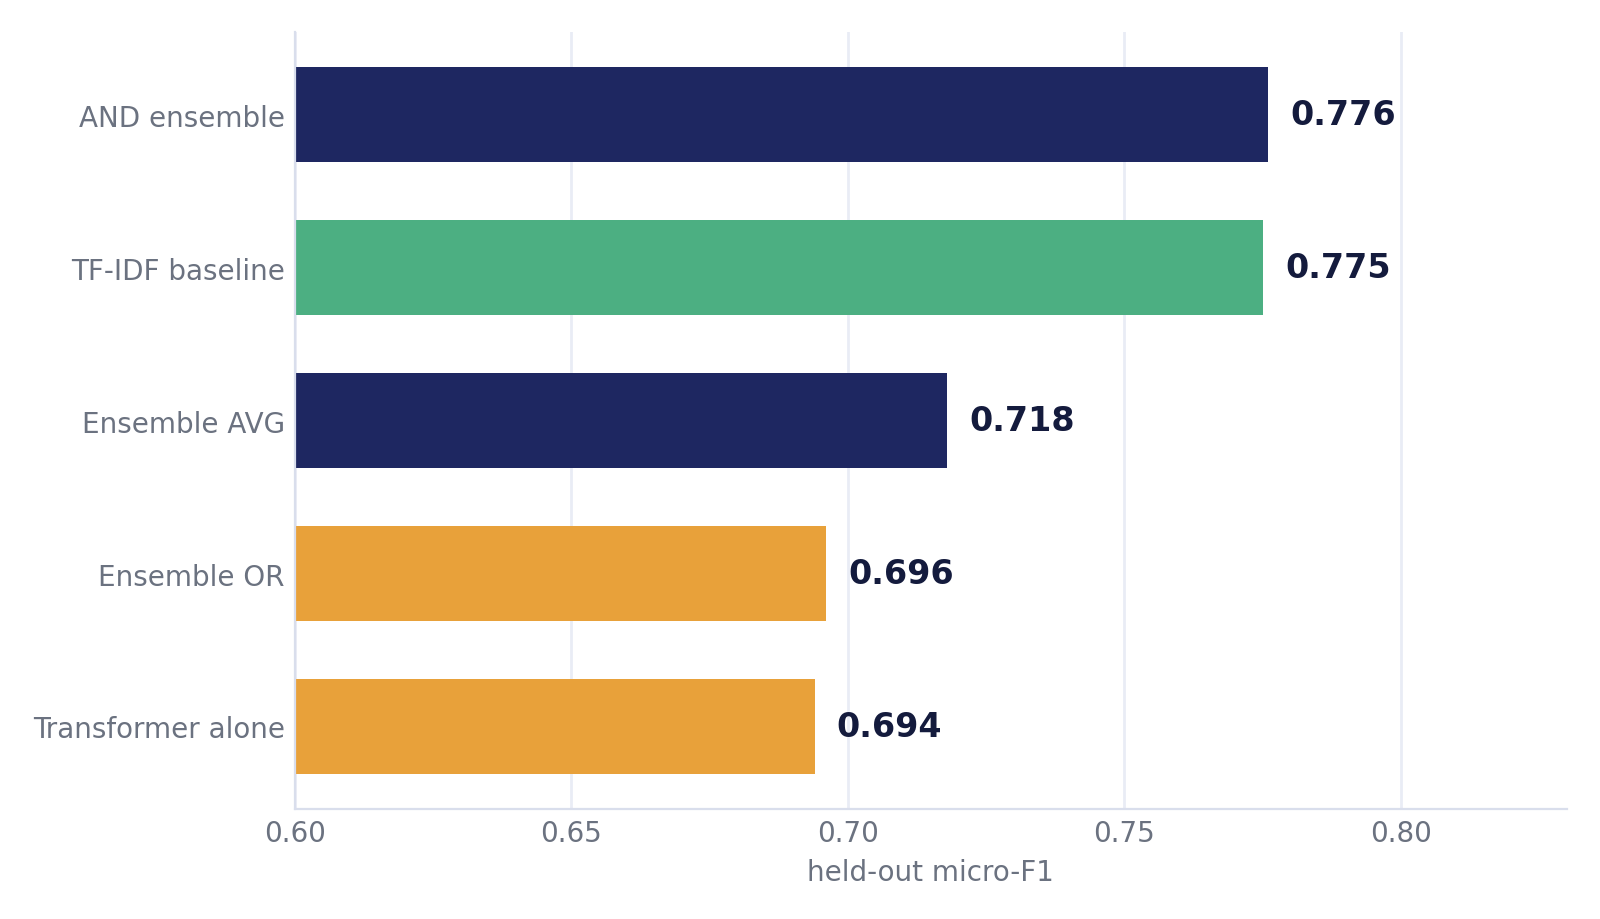
\includegraphics[width=\columnwidth]{chart_leaderboard.png}
\caption{Presence micro-F1 on the same 102 test contracts. In the first setup the transformer
trails the baseline by 0.082; with the whole window read and both models tuned on validation it
ties the baseline, and the ensemble leads it by a margin the bootstrap confirms.}
\label{fig:leaderboard}
\end{figure}

The re-run changed three things at once: input length, training contracts (327 instead of 408) and
tuning. The 256-token control separates them (Table~\ref{tab:v2ctrl}). Untuned, the 256-token model
scores 0.693, the same as the original 0.692, so the change of training contracts and epoch has no
measurable effect. With identical tuning, reading the whole window adds $+0.024$ micro-F1 untuned
($[+0.014,+0.035]$), $+0.036$ when both are tuned for micro-F1, and $+0.028$ micro-F2 when both are
tuned for recall ($[+0.015,+0.041]$), where the share of High-risk clauses found rises by 8.0 points
($[+3.4,+12.9]$). Tuning alone is not enough: at 256 tokens the tuned transformer still loses to the
tuned baseline by 0.024 ($[-0.041,-0.007]$). The first-setup gap came from two flaws, and closing
it took both fixes.

\begin{table}[!t]
\caption{Length-only control: 256 against 512 tokens}
\label{tab:v2ctrl}
\centering
\small
\setlength{\tabcolsep}{3pt}
\begin{tabular}{llcc}
\toprule
\textbf{Tuning} & \textbf{Model} & \textbf{256: F1 / F2} & \textbf{512: F1 / F2}\\
\midrule
None & Transformer & 0.693 / 0.815 & 0.717 / 0.842\\
\midrule
\multirow{2}{*}{F1} & Transformer & 0.761 / 0.800 & 0.797 / 0.836\\
 & Ensemble & 0.810 / 0.829 & 0.809 / 0.780\\
\midrule
\multirow{2}{*}{F2} & Transformer & 0.716 / 0.824 & 0.757 / 0.852\\
 & Ensemble & 0.777 / 0.826 & 0.783 / 0.861\\
\bottomrule
\end{tabular}
\end{table}

The ensemble's lead comes mainly from tuning: tuned for micro-F1 it scores 0.810 with the 256-token
transformer and 0.809 with the 512-token one. The window matters most for recall. With 256 tokens
neither recall-first configuration beats the tuned baseline on micro-F2; with 512 tokens both do
(the ensemble by $+0.029$, $[+0.018,+0.040]$). The re-run made many choices on only 81 validation
contracts, including up to 41 thresholds per model, so validation scores are optimistic (0.857 for
the tuned ensemble against 0.809 on test); the test scores remain clean because the test set played
no part in any choice.

\subsection{Risk-Weighted and Rare-Category Analysis}
\label{sec:risk}
Micro-F1 weights all 41 categories equally; the system's purpose does not.
Table~\ref{tab:risk} scores configurations from both setups within each risk band.

\begin{table}[!t]
\caption{Presence performance by risk band}
\label{tab:risk}
\centering
\small
\setlength{\tabcolsep}{4pt}
\begin{tabular}{llccc}
\toprule
\textbf{Band} & \textbf{Configuration} & \textbf{Prec.} & \textbf{Rec.} & \textbf{Missed}\\
\midrule
\multirow{8}{*}{\shortstack[l]{High\\(176 pos.)}}
 & \emph{First:} Transformer & 0.392 & 0.841 & 28\\
 & \emph{First:} TF--IDF      & 0.540 & 0.648 & 62\\
 & \emph{First:} AND          & 0.581 & 0.631 & 65\\
 & \emph{First:} OR           & 0.379 & 0.858 & 25\\
 & \emph{Re-run:} AND, F1     & 0.736 & 0.540 & 81\\
 & \emph{Re-run:} TF--IDF, F1 & 0.572 & 0.676 & 57\\
 & \emph{Re-run:} AVG, F2     & 0.515 & 0.869 & 23\\
 & \emph{Re-run:} Transf., F2 & 0.439 & \textbf{0.903} & \textbf{17}\\
\addlinespace
\multirow{3}{*}{\shortstack[l]{Medium\\(498 pos.)}}
 & \emph{First:} AND          & 0.655 & 0.679 & 160\\
 & \emph{First:} OR           & 0.424 & 0.930 & 35\\
 & \emph{Re-run:} Transf., F2 & 0.534 & 0.890 & 55\\
\addlinespace
\multirow{3}{*}{\shortstack[l]{Low\\(674 pos.)}}
 & \emph{First:} AND          & 0.923 & 0.902 & 66\\
 & \emph{First:} OR           & 0.792 & 0.967 & 22\\
 & \emph{Re-run:} Transf., F2 & 0.843 & 0.966 & 23\\
\bottomrule
\end{tabular}
\end{table}

\begin{figure}[!t]
\centering
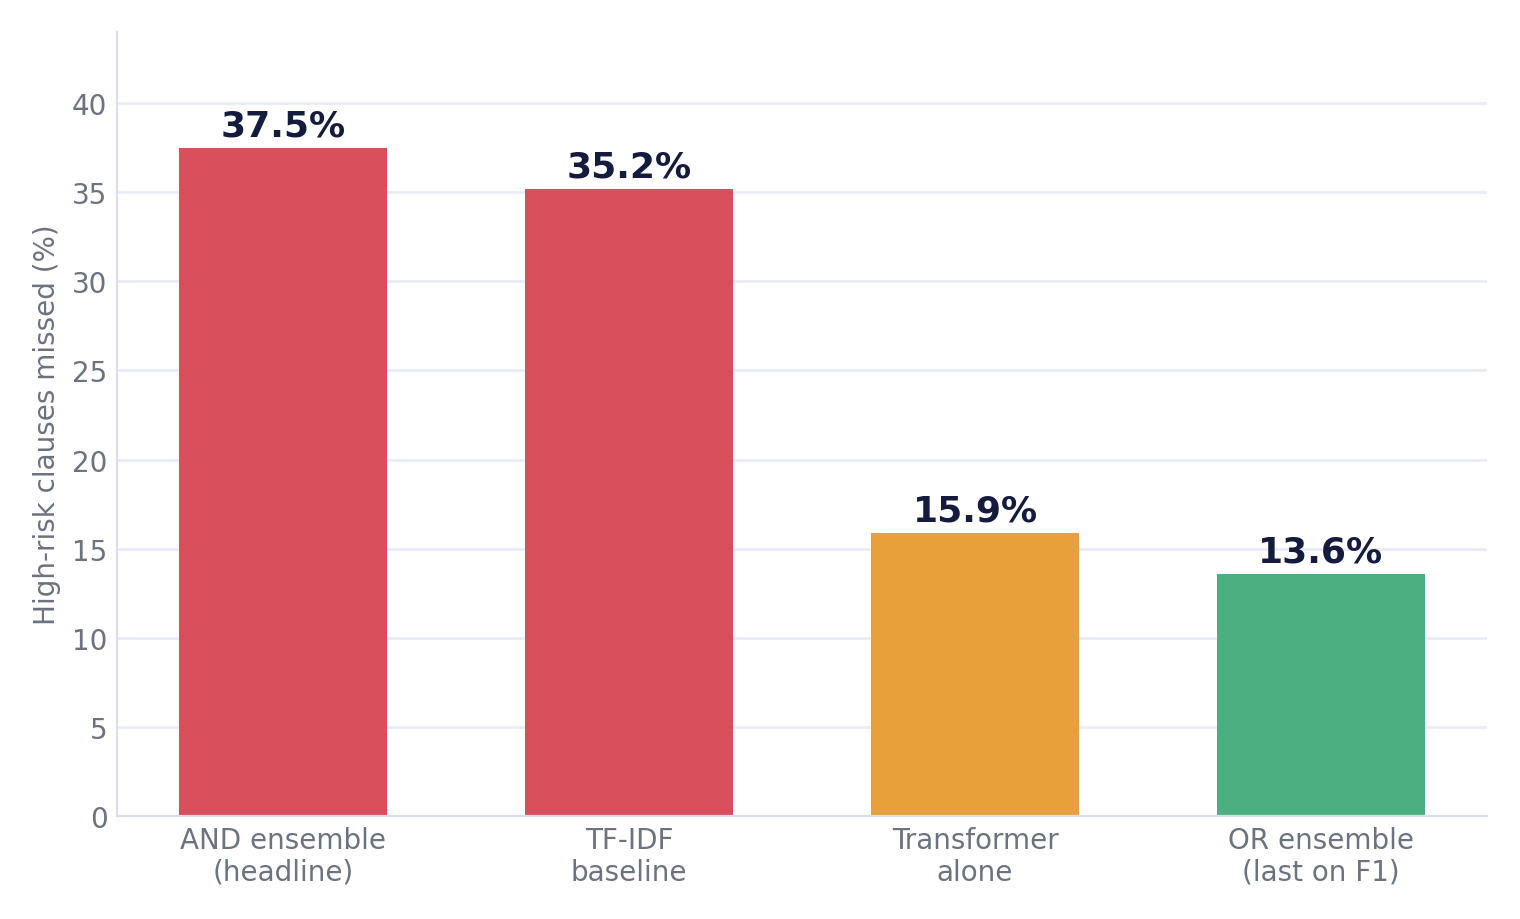
\includegraphics[width=\columnwidth]{chart_highrisk.png}
\caption{Share of the 176 high-risk test clauses missed by each configuration. In both setups the
configuration chosen for micro-F1 misses the most; the recall-first transformer chosen on
validation misses the fewest.}
\label{fig:highrisk}
\end{figure}

In the first setup, the configuration ranked first on aggregate micro-F1 misses \textbf{36.9\%} of
high-risk clauses, while the OR rule, ranked last, misses \textbf{14.2\%}. Half of the aggregate's
positives are low-risk categories such as dates, party names and governing law, where every model
scores about 0.9, so the metric is dominated by the clauses that matter least. Choosing OR after
seeing these test results would have been test-set selection, so the first setup reported this
only as a diagnosis. The re-run resolves it properly: the recall-first objective was fixed in
advance and every rule and threshold was chosen on validation. The same conflict reappears (the
micro-F1-optimal ensemble finds only 54.0\% of high-risk clauses), but the recall-first transformer
finds \textbf{90.3\%} at a micro-F1 of 0.757, and the recall-first ensemble finds 86.9\% at 0.783,
beating the first setup's headline configuration on both measures. The deployed application uses
the recall-first transformer.

The rare tail shows why. On the ten rarest categories (70 test positives) the first-setup AND rule
yields no F1 gain over the transformer alone (0.364 against 0.368): it buys 34.6 points of precision
with 30.0 points of recall, cuts detections from 39 of 70 to 18, and scores exactly zero on five of
the ten. Agreement is hardest to obtain where training data is thinnest. The re-run's recall-first
transformer finds 49 of the 70 (F1 0.460) and scores zero on only one of the ten, whereas the
re-run AND configuration again finds 18 and scores zero on five.

\subsection{Calibration}
The first-setup max-pooled score has an ECE of 0.205 and a Brier score of 0.195, and is
overconfident throughout: predictions above 0.9 correspond to the clause being present 72.6\% of
the time, and predictions in $[0.5,0.6)$ to 16.5\%. A maximum over dozens of windows is not a
probability-preserving operation, and nothing in training asked it to be. The re-run model's raw
score is no better (test ECE 0.206), and its validation-chosen thresholds of 0.96 (F1) and 0.88
(F2) show that its scores still bunch near 1. An isotonic map fitted on the 81 validation contracts
and applied unchanged to the test set lowers ECE to 0.016 and the Brier score to 0.091; Platt
scaling reaches 0.084. Because the map is monotone it changes no detection. On the test set,
contracts with a raw score of at least 0.99 contained the clause 99.0\% of the time, and those
between 0.90 and 0.95 only 32.3\% of the time, a distinction the raw score hides.

\begin{figure}[!t]
\centering
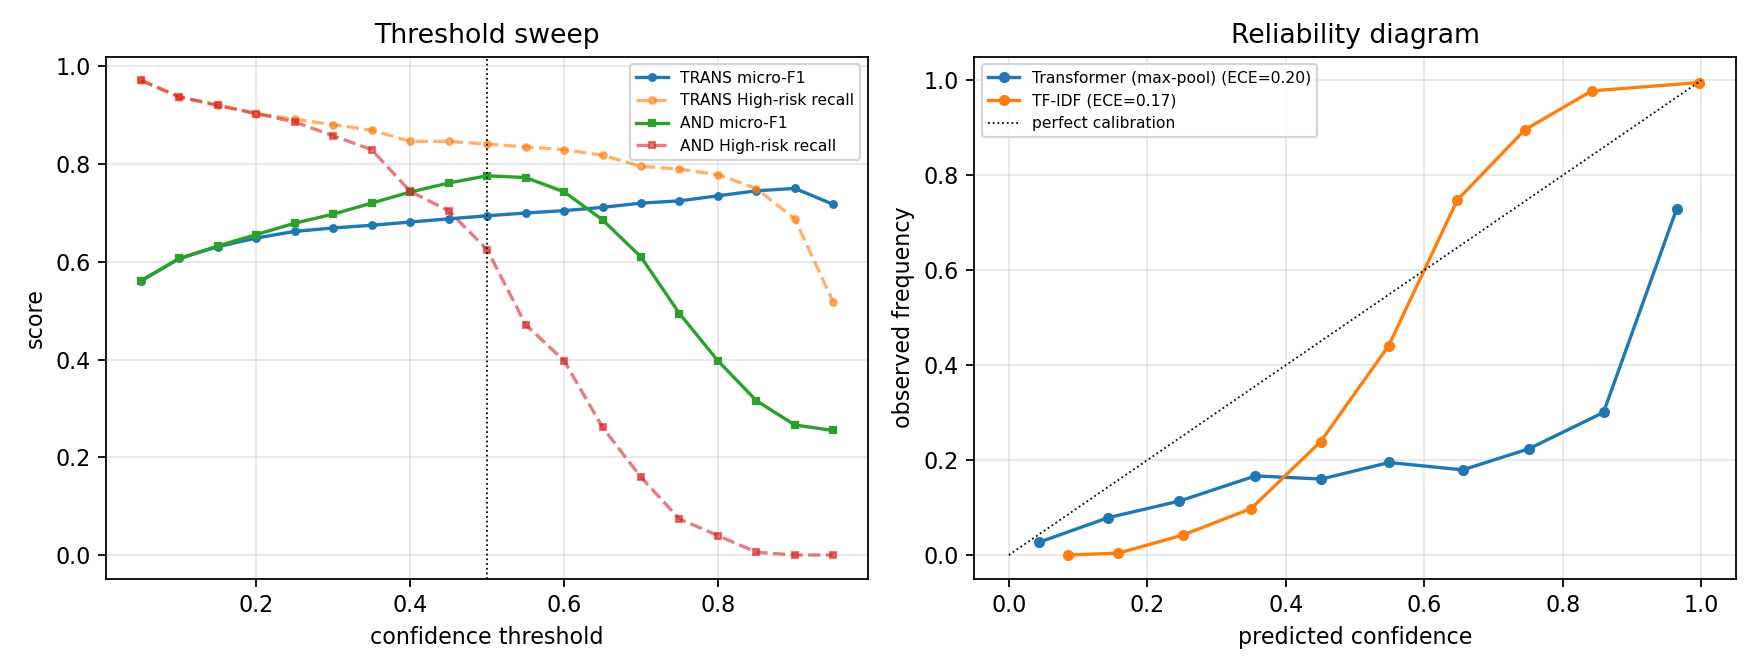
\includegraphics[width=\columnwidth]{threshold_calibration.png}
\caption{First setup: threshold sweep (left) and reliability diagram (right). The default 0.5
boundary is a poor operating point for the max-pooled transformer, and the raw score it thresholds
is not calibrated.}
\label{fig:cal}
\end{figure}

\subsection{Span Extraction and Plain-Language Generation}
\label{sec:summ}
Given a window centred on the answer, the first span model reaches a token-F1 of 0.764 with a
contract-clustered 95\% interval of $[0.743,0.782]$, and 82.8\% of predictions overlap the gold
span at F1 $\geq 0.5$. The clustered
interval is roughly twice the width obtained by resampling clauses independently
($[0.752,0.775]$), which is the practical cost of ignoring within-contract correlation.

CUAD contains no plain-English rewrites, so the 41 generation targets were author-written and every
test clause is scored against one of only 41 unique strings. To separate template reproduction from
summarization we scored the same 150 held-out clauses against a second, clause-specific reference set
drafted independently of the model (Table~\ref{tab:summ}).

\begin{table}[!t]
\caption{ROUGE-L under two reference sets, same 150 clauses}
\label{tab:summ}
\centering
\small
\begin{tabular}{llc}
\toprule
\textbf{System} & \textbf{References} & \textbf{ROUGE-L}\\
\midrule
Fine-tuned FLAN-T5 & 41 templates    & 0.775\\
Fine-tuned FLAN-T5 & clause-specific & 0.116\\
Zero-shot FLAN-T5  & clause-specific & 0.299\\
\emph{Template alone, no model} & clause-specific & 0.115\\
\bottomrule
\end{tabular}
\end{table}

The fine-tuned model emits one of the 41 templates verbatim on 100\% of inputs, the correct one 70\%
of the time, and a constant lookup table matches its score. The task became 41-way classification and
the metric did not register the change. A template-emitting model cannot hallucinate in the usual
sense; it fails instead by producing fluent, confident text about a different provision, which is
undetectable from the output alone.

\subsection{End-to-End Evaluation}
\label{sec:e2e}
Running all stages in series over the 1,348 gold clauses in the test contracts gives
Table~\ref{tab:e2e}. A clause survives only if its category is detected, the span extracted from the
\emph{selected} window overlaps the gold clause at token-F1 $\geq 0.5$, and the risk label is
correct.

\begin{table}[!t]
\caption{End-to-end survival over 1,348 gold clauses}
\label{tab:e2e}
\centering
\small
\setlength{\tabcolsep}{4pt}
\begin{tabular}{lcc}
\toprule
\textbf{Stage} & \textbf{First (AND)} & \textbf{App (F2)}\\
\midrule
Presence detected       & 1,057 (78.4\%) & 1,253 (93.0\%)\\
Span overlap $\geq 0.5$ & 296 (22.0\%)   & 298 (22.1\%)\\
Risk label correct      & 296 (22.0\%)   & 298 (22.1\%)\\
\midrule
95\% CI (contracts)     & $[19.8, 24.2]$ & $[19.7, 24.6]$\\
\addlinespace
Selected window correct & 69.1\%         & 82.6\%\\
\quad then span found   & 39.6\%         & 28.0\%\\
\bottomrule
\end{tabular}
\end{table}

Multiplying the component figures predicts about 65\% for the first setup and 77\% for the
application setting; both deliver less than a third of that. Two causes account for the loss. The
first is a detector reused as a locator: max-pooling was trained to answer whether a window contains
a clause, not which window does, and the first-setup model's top window misses the clause 30.9\% of
the time. Reading the whole window cuts this to 17.4\%. The second is the re-centring used at
training time, which is legitimate with respect to leakage but narrows the distribution the span
model can read. Given a correct window, extraction succeeds 39.6\% of the time in the first setup
and 28.0\% in the application setting, against 82.8\% in isolation, and mean token-F1 falls from
0.764 to 0.383 (0.350). Clause position explains the drop. Because the first model read only the
first half of each window, its correct windows had the clause in the second half only 8.9\% of the
time, against 35.8\% for the full-window model. In the first half the span model succeeds about
equally for both (41.7\% and 40.7\%); in the second half it succeeds 18.5\% and 5.4\% of the time.
The whole drop from 39.6\% to 28.0\% therefore comes from clauses the first model could not see,
and with the window fixed, the span model's positional bias became the main loss.

The retrained span model (Section~\ref{sec:stage2}) removes it. It uses the same backbone, learning
rate and two epochs, 384 tokens, and 11,967 chunks from 6,000 clauses of the 327 fit contracts. The
epoch and the decoding (each chunk's best answer scored against its ``no answer'' score, at most 120
tokens) were chosen on the 81 validation contracts, where it extracts 63.4\% of detected clauses
against 20.9\% for the first model. On the test set (Table~\ref{tab:spanv2}), given the right window
it succeeds 76.4\% of the time, with no position effect (76.2\% in the first half, 76.8\% in the
second), and end-to-end survival under the application setting rises from 22.1\% to 59.6\%. On a
plain window that contains the clause the first model reaches a mean token-F1 of only 0.366, far
below its centred-window 0.764, while the retrained model reaches 0.779. Survival now follows
$93.0\% \times 82.6\% \times 76.4\% = 58.7\%$, plus 12 clauses recovered from a wrong window. Of
the 545 clauses still lost, 95 are never detected, 206 lie outside the selected window and 244 are
missed inside it, so the two causes now cost about the same. No extra parameters were needed for
either fix.

\begin{table}[!t]
\caption{First and retrained span model, same detections and windows}
\label{tab:spanv2}
\centering
\small
\setlength{\tabcolsep}{4pt}
\begin{tabular}{lcc}
\toprule
 & \textbf{First} & \textbf{Retrained}\\
\midrule
Survive all stages (app setting) & 22.1\% & \textbf{59.6\%}\\
\quad 95\% CI (contracts) & $[19.7, 24.6]$ & $[57.0, 62.2]$\\
Span found, right window & 28.0\% & 76.4\%\\
\quad clause in first half & 40.7\% & 76.2\%\\
\quad clause in second half & 5.4\% & 76.8\%\\
Survive all stages (balanced) & 19.7\% & 50.7\%\\
Token-F1, plain right window & 0.366 & 0.779\\
\bottomrule
\end{tabular}
\end{table}

The application quotes the paragraph around the extracted answer and highlights the answer in it.
Counting a quote as correct when it contains at least half of the clause's words, 77.2\% of
detected clauses receive a correct quote, against 75.3\% when the paragraph is chosen by the presence
model, the method the application used before (the choice was made on validation). Over all gold
clauses that is 71.7\% ($[69.0, 74.5]$).

\subsection{Limitations}
\label{sec:limits}
The re-run tuned up to 41 thresholds per model on 81 validation contracts, so some per-category
thresholds fit noise; this inflates validation scores but not test scores. The seed, training-budget
and split controls were run on the first setup and have not been repeated for the re-run model or
the retrained span model, and
the ensemble's own split variance is unmeasured. ROUGE-L measures its reference set rather than the
task, as Section~\ref{sec:summ} demonstrates directly, and micro-F1 does not measure user harm, as
Section~\ref{sec:risk} demonstrates. The risk levels are our own, and a different assignment would
change the risk-weighted numbers. The application has not been tested with users. All results come
from 510 US commercial contracts drawn from SEC filings, in English; no contract outside that corpus
has been evaluated. Three seeds is a small sample for a standard deviation, and per-category
statistics on the rare tail are not meaningful individually.

\section{Engineering Considerations}
Training the first-setup presence transformer took 49.8 minutes on the target laptop, the
full-data control 140.7 minutes, and the re-run 191 minutes, with another 198 minutes to score every
validation and test window; the summarizer trained on CPU in about 8 minutes, and the retrained span model in 46.2 minutes. DeBERTa-v3 produced NaN
gradients on the Metal backend and was replaced by DistilBERT. Gradient norms logged every 100 steps
exceeded the clipping limit of 1.0 at every logged step of the October DistilBERT runs and at 98.4\%
of logged points in the full-data run, so the nominal learning rate overstates the step size actually
taken.

Sparse attention was rejected on cost, and that cost was measured rather than asserted.
Longformer-base at 4,096 tokens requires 14.71\,GB for a single training step at batch size 1 on a
16\,GB machine, which fits and contradicts our own earlier claim, but 20.75\,GB at batch size 2,
where paging makes the step 8.4 times slower for twice the work. At 258\,s per step the two-epoch
presence schedule would take approximately 136 days against about 50 minutes for DistilBERT. On the
inference side, scanning one median contract for all 41 categories takes 10.6\,s with DistilBERT
against 454\,s with Longformer.

The deployed application runs all inference locally on CPU. With the full-window model, a
median-length test contract takes 64.4\,s and the worst case 87.1\,s at a peak memory of 1.93\,GB,
about twice the first setup's 30.1\,s because each window now carries twice as much text. A
30-window cap bounds latency but reads only the first 45,500 characters, and 38.4\% of CUAD
contracts exceed that, so clauses beyond the cap cannot be detected, a limitation invisible in every
offline metric reported above.

\section{Conclusion and Future Work}
On a strict held-out protocol, a full-document lexical baseline first appeared to beat a windowed
transformer at clause presence classification, and the result survived controls for training
budget, random seed, aggregation rule and decision threshold. All of those controls shared a
256-token limit that hid half of every window. With the whole window read and both models tuned on
the same validation split, the transformer ties the baseline and their ensemble beats it (0.809,
lead $[+0.011,+0.037]$). In both setups the configuration that maximizes aggregate micro-F1 is the
worst available choice for the clauses carrying the highest risk, and a recall-first objective
fixed before testing finds 90.3\% of them. The assembled pipeline first retained only 22.1\% of gold clauses where its component scores
predicted about 77\%; both causes lay in our own setup, and fixing them raises survival to 59.6\%. We suggest that a comparison is fair only
when both sides read the same evidence and are tuned the same way, that a margin should be compared
against seed and split variance as well as a bootstrap interval, and that pipeline-level survival
and a purpose-weighted metric belong alongside component scores in any system of this kind.

Future work: a locator trained for locating rather than a detector reused as one, and further
training of the span model, which target the two remaining losses; a tuning objective that weights high-risk categories; repeating the seed and split controls
for the re-run model, with cross-validation; a clause-diverse generation target set; dense retrieval;
a user study of the application; and evaluation on contracts drawn from outside CUAD.

\section*{Acknowledgment}
The authors thank Utsha Kumar Roy for requiring a strict held-out evaluation protocol, which shaped
how this work reports its results.

\begin{thebibliography}{99}
\bibitem{cuad} D. Hendrycks, C. Burns, A. Chen, and S. Ball, ``CUAD: An expert-annotated NLP dataset for legal contract review,'' in \emph{Proc. NeurIPS Datasets and Benchmarks}, 2021.
\bibitem{squad} P. Rajpurkar, J. Zhang, K. Lopyrev, and P. Liang, ``SQuAD: 100,000+ questions for machine comprehension of text,'' in \emph{Proc. EMNLP}, 2016, pp. 2383--2392.
\bibitem{squad2} P. Rajpurkar, R. Jia, and P. Liang, ``Know what you don't know: Unanswerable questions for SQuAD,'' in \emph{Proc. ACL}, 2018, pp. 784--789.
\bibitem{legalbert} I. Chalkidis \emph{et al.}, ``LEGAL-BERT: The muppets straight out of law school,'' in \emph{Findings of EMNLP}, 2020, pp. 2898--2904.
\bibitem{lexglue} I. Chalkidis \emph{et al.}, ``LexGLUE: A benchmark dataset for legal language understanding in English,'' in \emph{Proc. ACL}, 2022.
\bibitem{longformer} I. Beltagy, M. E. Peters, and A. Cohan, ``Longformer: The long-document transformer,'' \emph{arXiv:2004.05150}, 2020.
\bibitem{mil} O. Maron and T. Lozano-P\'erez, ``A framework for multiple-instance learning,'' in \emph{Proc. NIPS}, 1998, pp. 570--576.
\bibitem{t5} C. Raffel \emph{et al.}, ``Exploring the limits of transfer learning with a unified text-to-text transformer,'' \emph{JMLR}, vol. 21, no. 140, pp. 1--67, 2020.
\bibitem{flan} H. W. Chung \emph{et al.}, ``Scaling instruction-finetuned language models,'' \emph{JMLR}, vol. 25, no. 70, pp. 1--53, 2024.
\bibitem{manor} L. Manor and J. J. Li, ``Plain English summarization of contracts,'' in \emph{Proc. Natural Legal Language Processing Workshop}, 2019, pp. 1--11.
\bibitem{maynez} J. Maynez, S. Narayan, B. Bohnet, and R. McDonald, ``On faithfulness and factuality in abstractive summarization,'' in \emph{Proc. ACL}, 2020, pp. 1906--1919.
\bibitem{factcc} W. Kry\'sci\'nski, B. McCann, C. Xiong, and R. Socher, ``Evaluating the factual consistency of abstractive text summarization,'' in \emph{Proc. EMNLP}, 2020, pp. 9332--9346.
\bibitem{rouge} C.-Y. Lin, ``ROUGE: A package for automatic evaluation of summaries,'' in \emph{Text Summarization Branches Out}, 2004, pp. 74--81.
\bibitem{bertscore} T. Zhang, V. Kishore, F. Wu, K. Q. Weinberger, and Y. Artzi, ``BERTScore: Evaluating text generation with BERT,'' in \emph{Proc. ICLR}, 2020.
\bibitem{calibration} C. Guo, G. Pleiss, Y. Sun, and K. Q. Weinberger, ``On calibration of modern neural networks,'' in \emph{Proc. ICML}, 2017, pp. 1321--1330.
\bibitem{distilbert} V. Sanh, L. Debut, J. Chaumond, and T. Wolf, ``DistilBERT, a distilled version of BERT,'' in \emph{Proc. EMC$^2$ Workshop, NeurIPS}, 2019.
\end{thebibliography}

\end{document}
